\documentclass[12pt]{article}
\pagestyle{empty}
\usepackage{graphicx}

\title{pipeComp - Main figures}

\date{\today}


\begin{document}
\maketitle

\begin{figure}
    \centering
    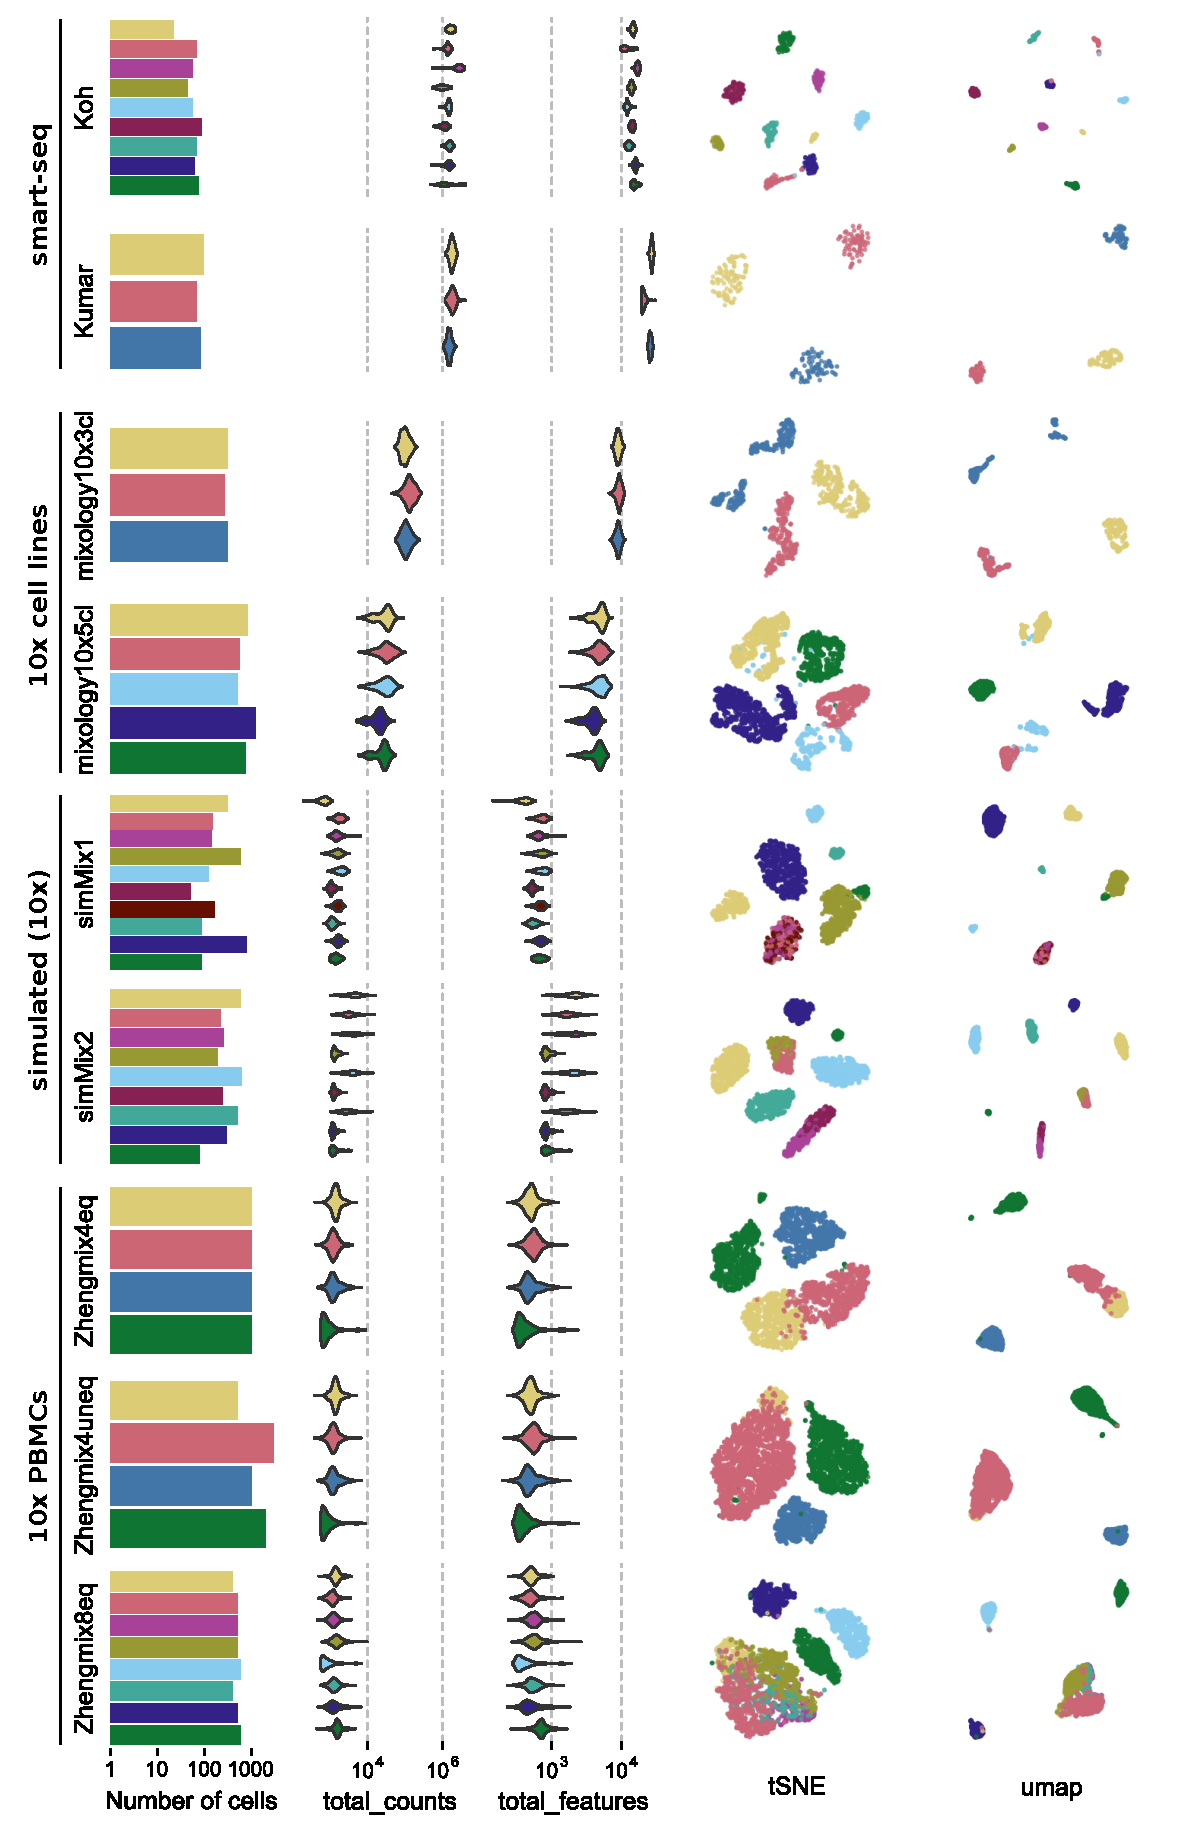
\includegraphics[width=\textwidth,keepaspectratio]{dataset_description}
    \caption{\textbf{Overview of the benchmark datasets used.}}
    \label{fig:figure1}
\end{figure}

\begin{figure}
    \centering
    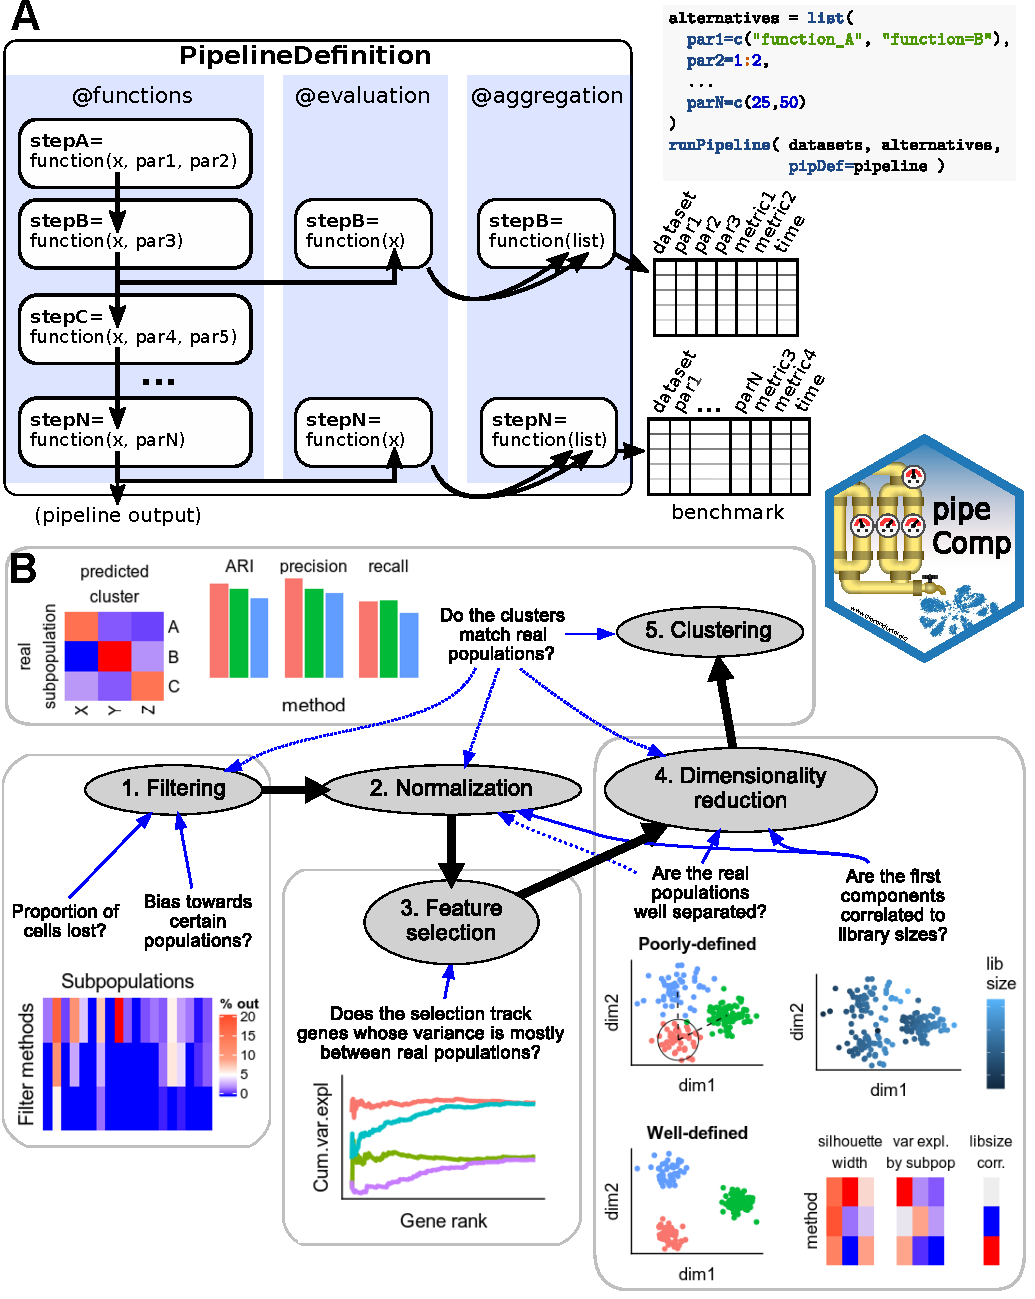
\includegraphics[scale=0.75, keepaspectratio]{main_figures/pipeline_explanation.pdf}
    \caption{\textbf{Overview of the \textit{pipeComp} framework and its application to a scRNAseq clustering pipeline. A:} The package is built around a \texttt{PipelineDefinition} S4 class which defines a set of functions to be executed consecutively, as well as optional evaluation functions for each step. Each step can accept a number of parameters whose alternative values are provided as a list. All (or subsets of) combinations of parameters can then be simultaneously ran and evaluated using the \texttt{runPipeline} function. \textbf{B:} Scheme representing the application of \textit{pipeComp} to evaluate a range of methods that are commonly used in scRNAseq studies and some of the metrics monitored at various steps.}
    \label{fig:figure2}
\end{figure}


\begin{figure}
    \centering
    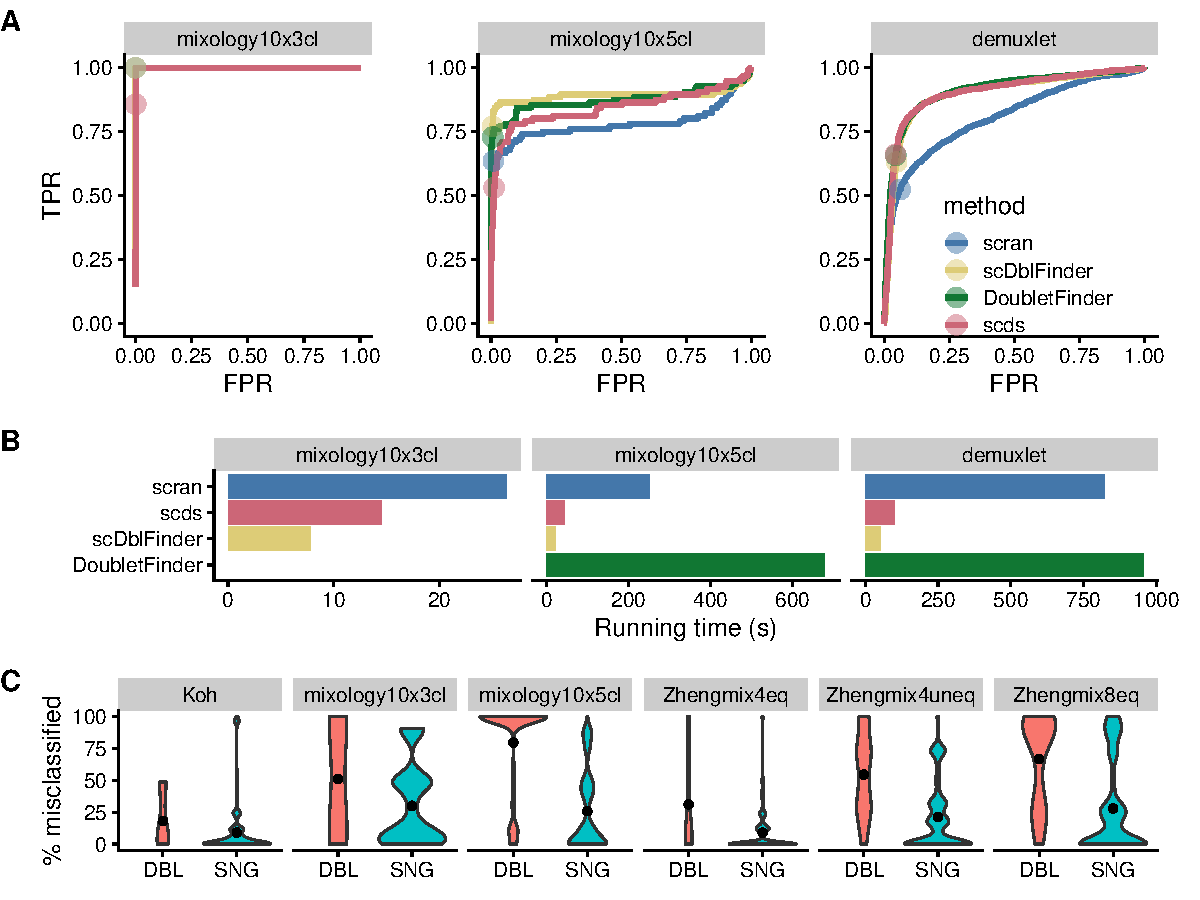
\includegraphics[scale=0.85, keepaspectratio]{{main_figures/doublets.pdf}}
    \caption{\textbf{Identification of doublet cells. A:} Receiver operating characteristic (ROC) curves of the tested doublet detection methods for three datasets with SNP-identified doublets. Dots indicate threshold determined by the true number of doublets. \textbf{B:} Running time of the different methods (\textit{DoubletFinder} failed on one of the datasets). \textbf{C:} Rate of misclassification of the cells identified by \textit{scDblFinder} as doublets (DBL) or singlets (SNG), across a large range of clustering analysis. Even in datasets which should not have neotypic doublets, the cells identified as such tend to be misclassified.    \label{fig:figure3}}
\end{figure}



\begin{figure}
    \centering
    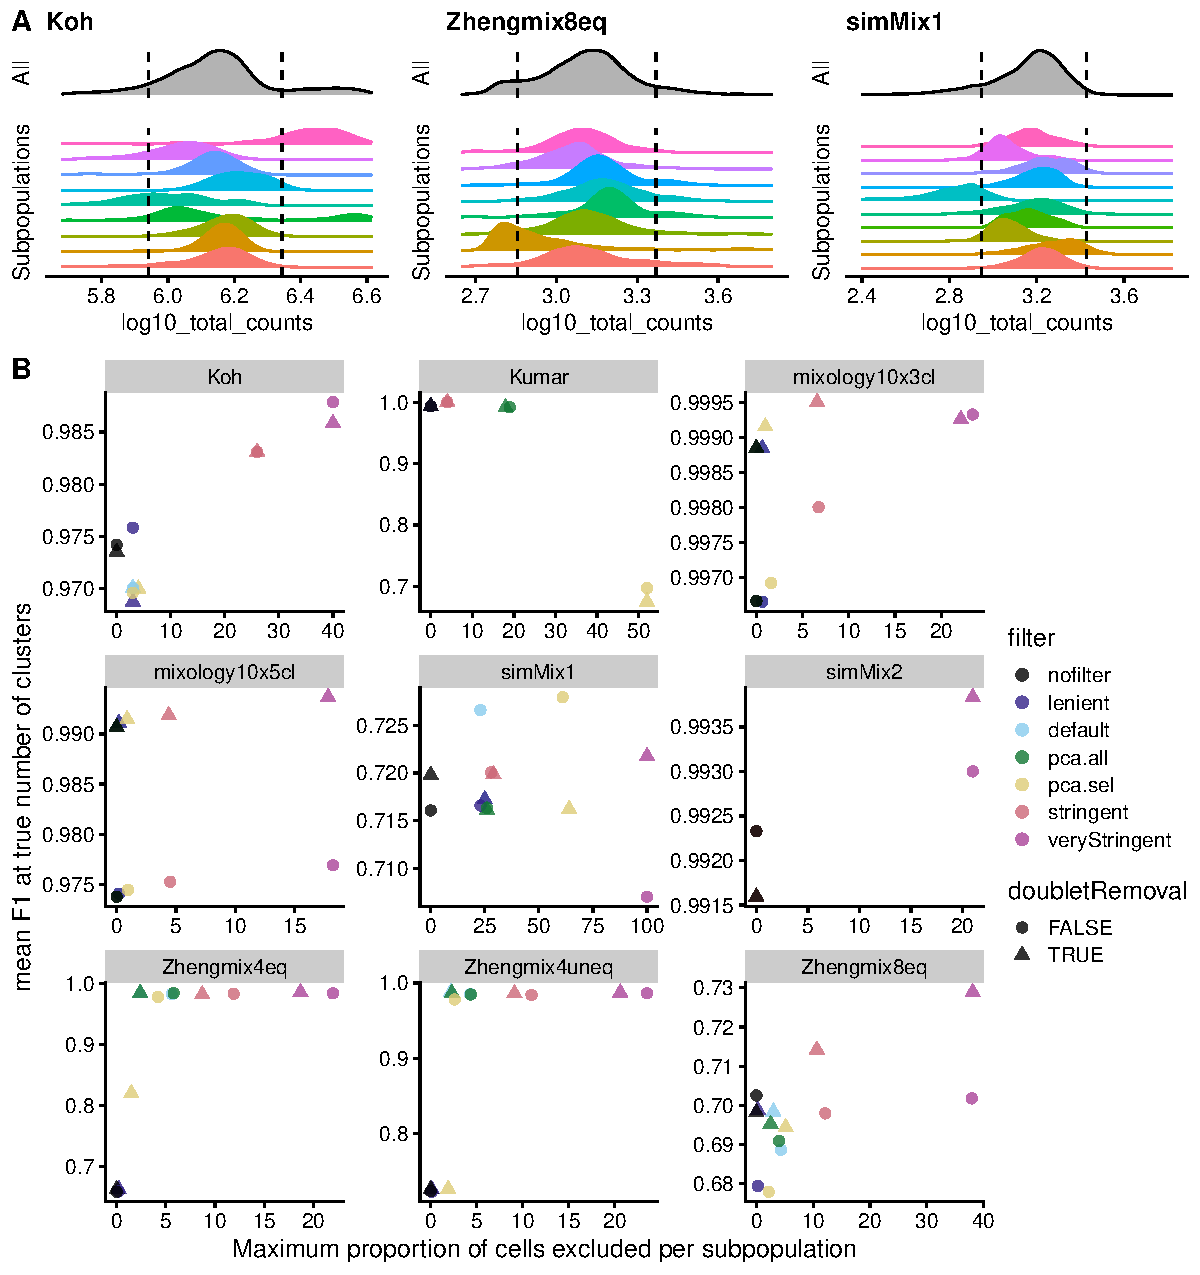
\includegraphics[scale=0.72, keepaspectratio]{{main_figures/filtering.pdf}}
    \caption{\textbf{Effect of filtering on cell subpopulation structure and clustering. A:} Filtering on the basis of distance to the whole distribution can lead to strong bias against certain subpopulations. The dashed line indicates a threshold of 2.5 median absolute deviations (MADs) from the median of the overall population. \textbf{B:} Relationship between the maximum subpopulation exclusion rate and the average clustering accuracy per subpopulation across various filtering strategies. Of note, doublet removal appears to be desirable even when, due to the design, there are no heterotypic doublets in the data. The PCA methods refer to multivariate outlier detected as implemented in \textit{scater} (see Methods for details).}
    \label{fig:figure4}
\end{figure}



\begin{figure}
    \centering
    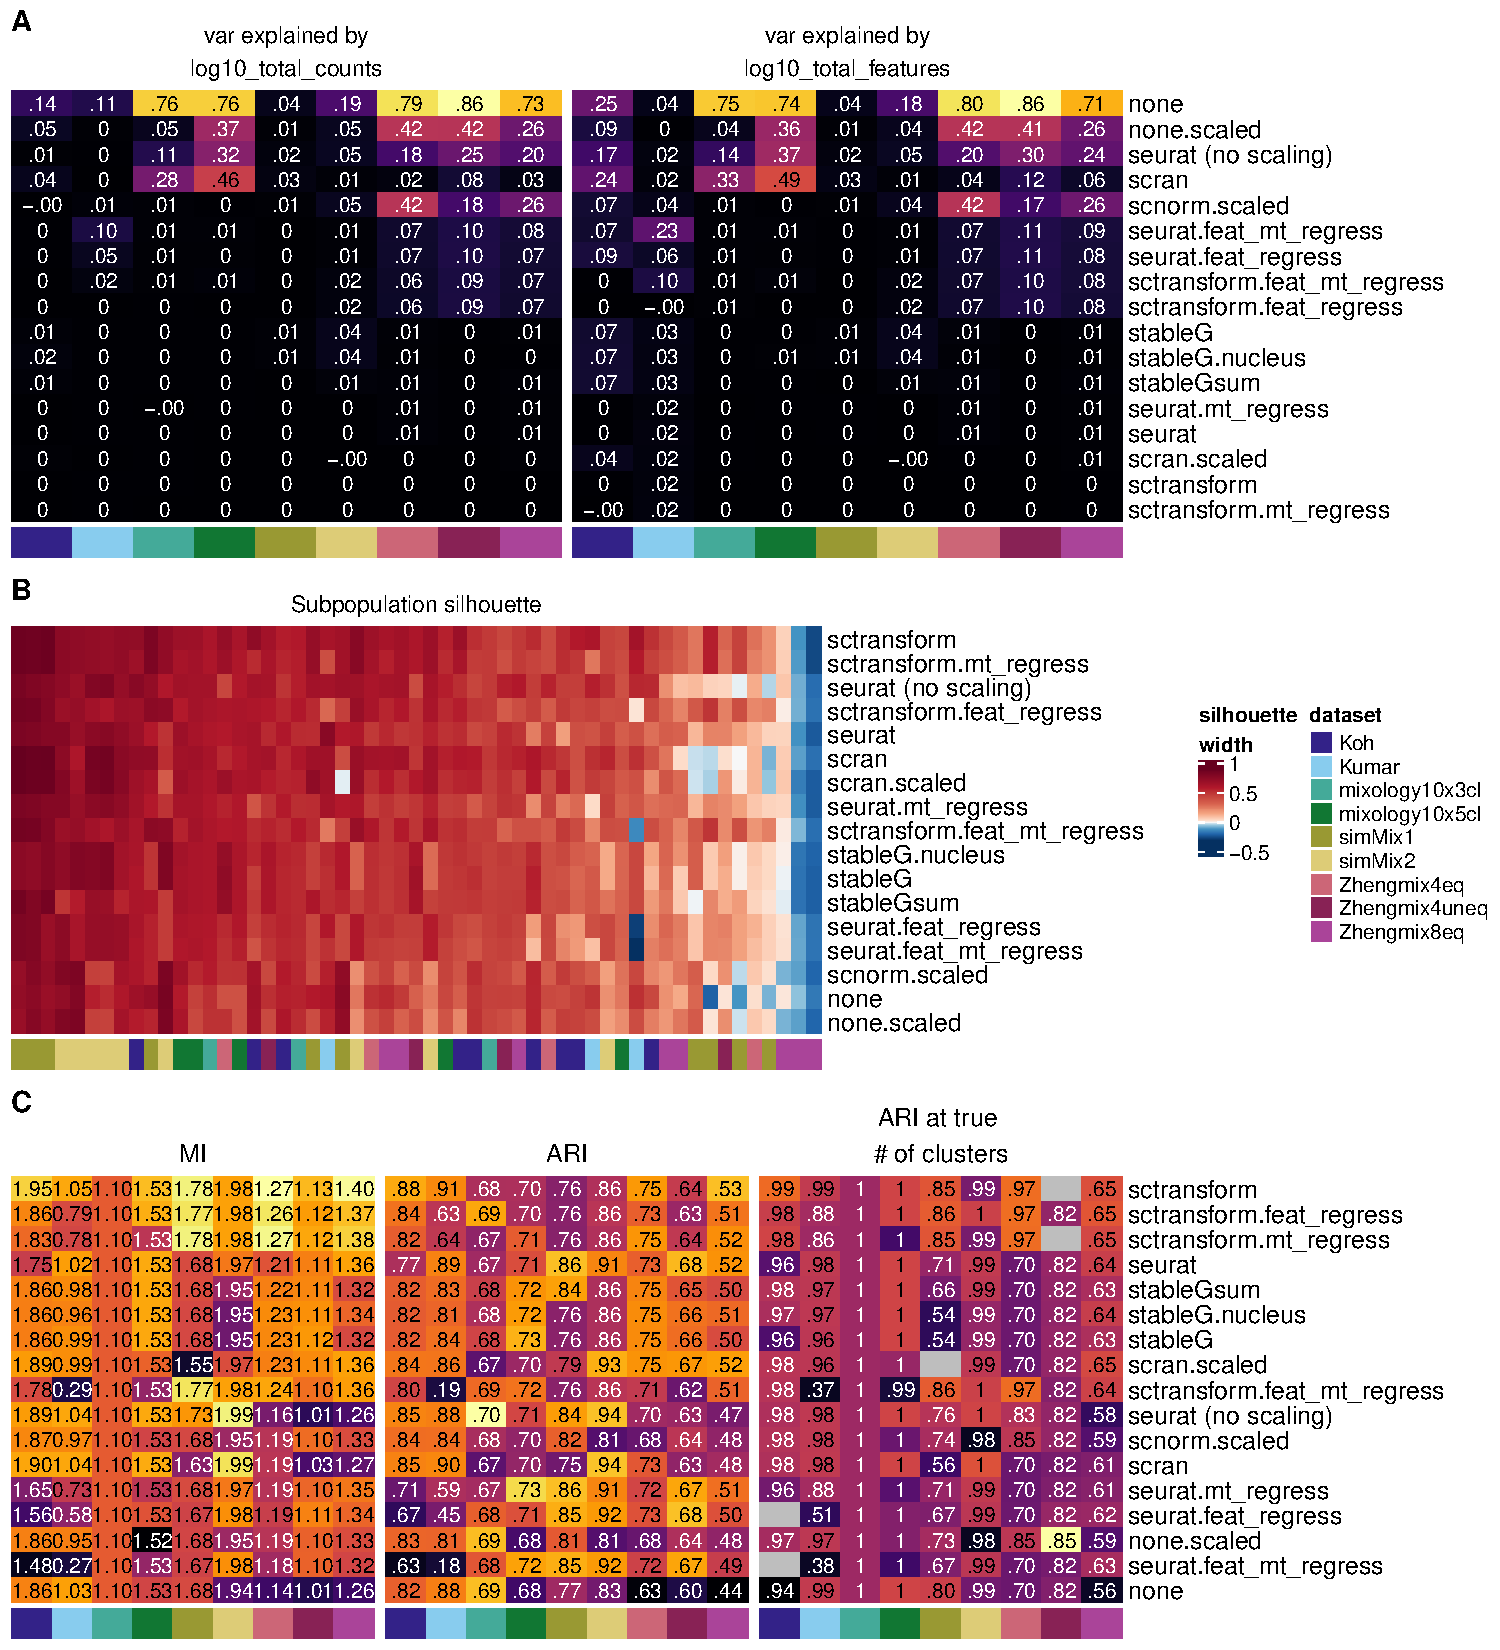
\includegraphics[scale=0.65, keepaspectratio]{{main_figures/normalization.pdf}}
    \caption{\textbf{Evaluation of normalization procedures.} \textbf{A:} Variance in PC1 explained by library size (left) and detection rate (right) after accounting for subpopulation differences. \textbf{B:} Average silhouette width per true subpopulation, where higher silhouette width means a higher separability. \textbf{C:} Clustering accuracy (\textit{Seurat} clustering), measured by mutual information (MI), Adjusted Rand Index (ARI) and ARI at the true number of cluster. 'feat_regress', 'mt_regress' and 'feat_mt_regress' respectively stand for the regressing out of the number of features, the proportion of mitochondrial reads, or both during scaling. }
    \label{fig:figure5}
\end{figure}



\begin{figure}
    \centering
    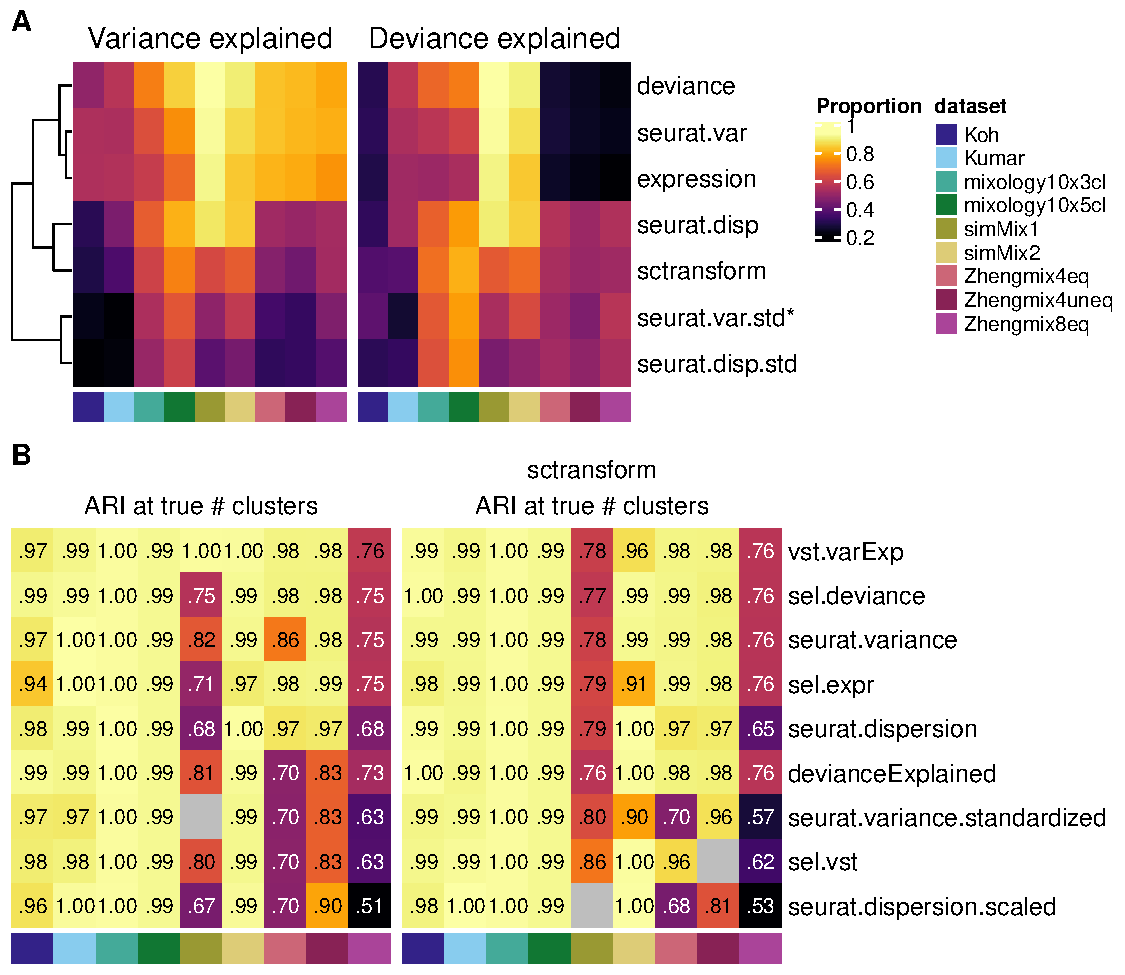
\includegraphics[scale=0.65]{{main_figures/selection.pdf}}
    \caption{\textbf{Evaluation of feature selection methods. A:} Ability of different feature ranking methods to capture genes with a high proportion of variance (left) or deviance (right) explained by real subpopulations. The asterisk denotes the default Seurat method. \textbf{B:} Accuracy of clusterings (at the true number of clusters) when selecting 1000 genes using the given methods. Based on standard \textit{Seurat} normalization (left) or \textit{sctransform} (right). The  \textit{vst.varExp} and \textit{devianceExplained} methods correspond to the estimates used in \textbf{A} to evaluate the selection methods and were included here only for validation purpose.}
    \label{fig:figure6}
\end{figure}



\begin{figure}
    \centering
    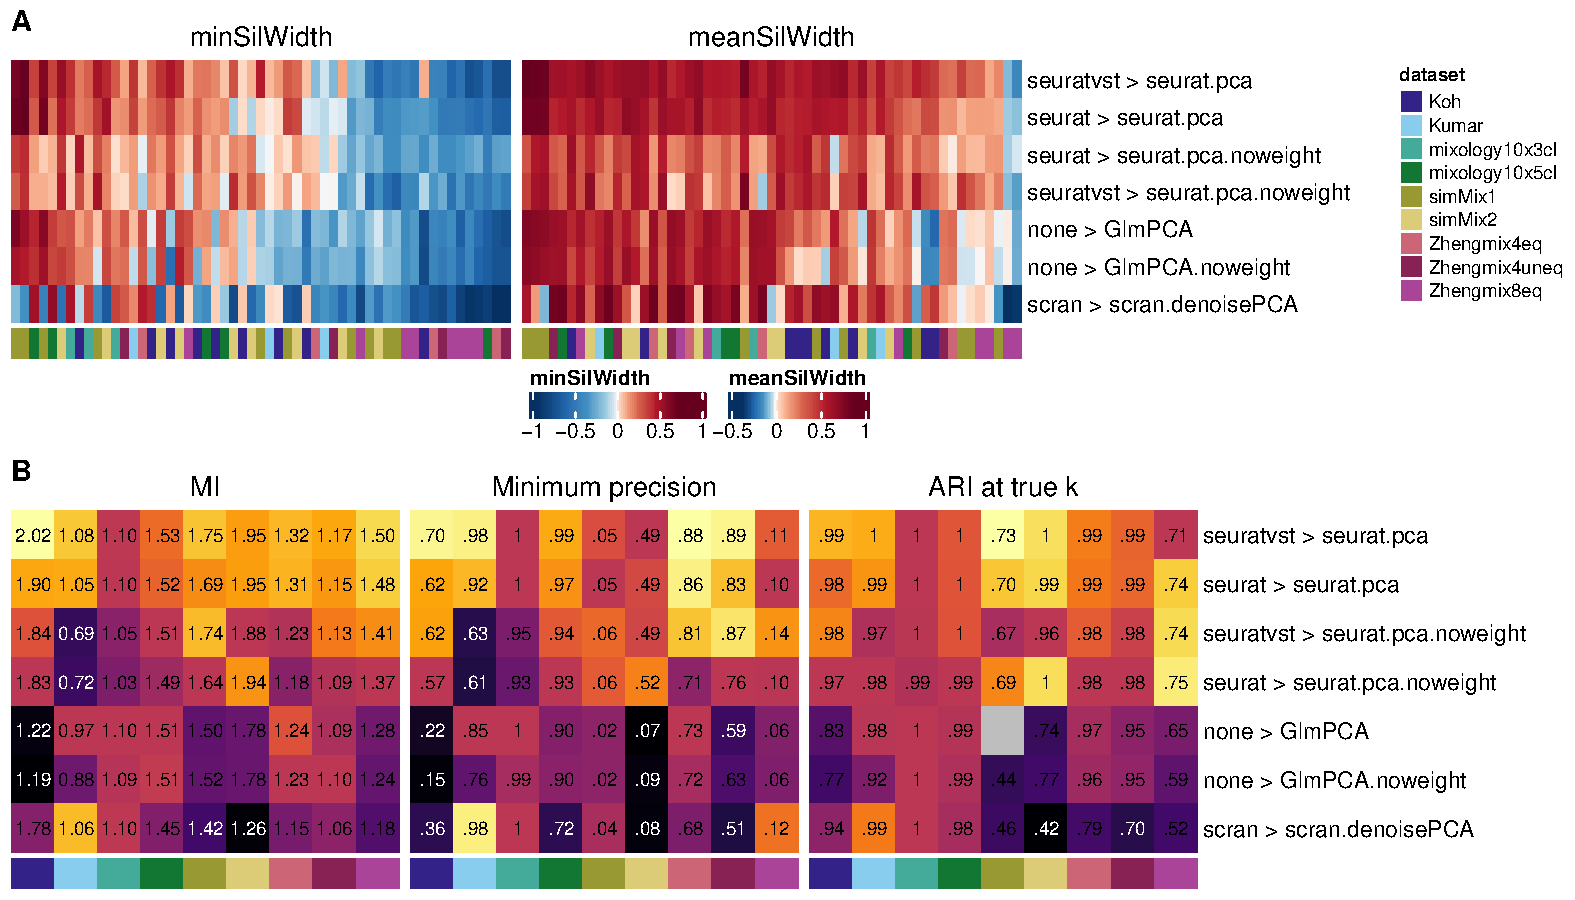
\includegraphics[scale=0.50, keepaspectratio]{{main_figures/dr.pdf}}
    \caption{\textbf{Evaluation of common dimensionality reduction methods. A:} Average silhouette width per subpopulation resulting from combinations of normalization and dimension reductions. \textbf{B:} Clustering accuracy, mean proportion of the variance in the first 5 components explained by real subpopulations (center), and median ARI of the resulting clustering (right).}
    \label{fig:figure7}
\end{figure}



\begin{figure}
    \centering
    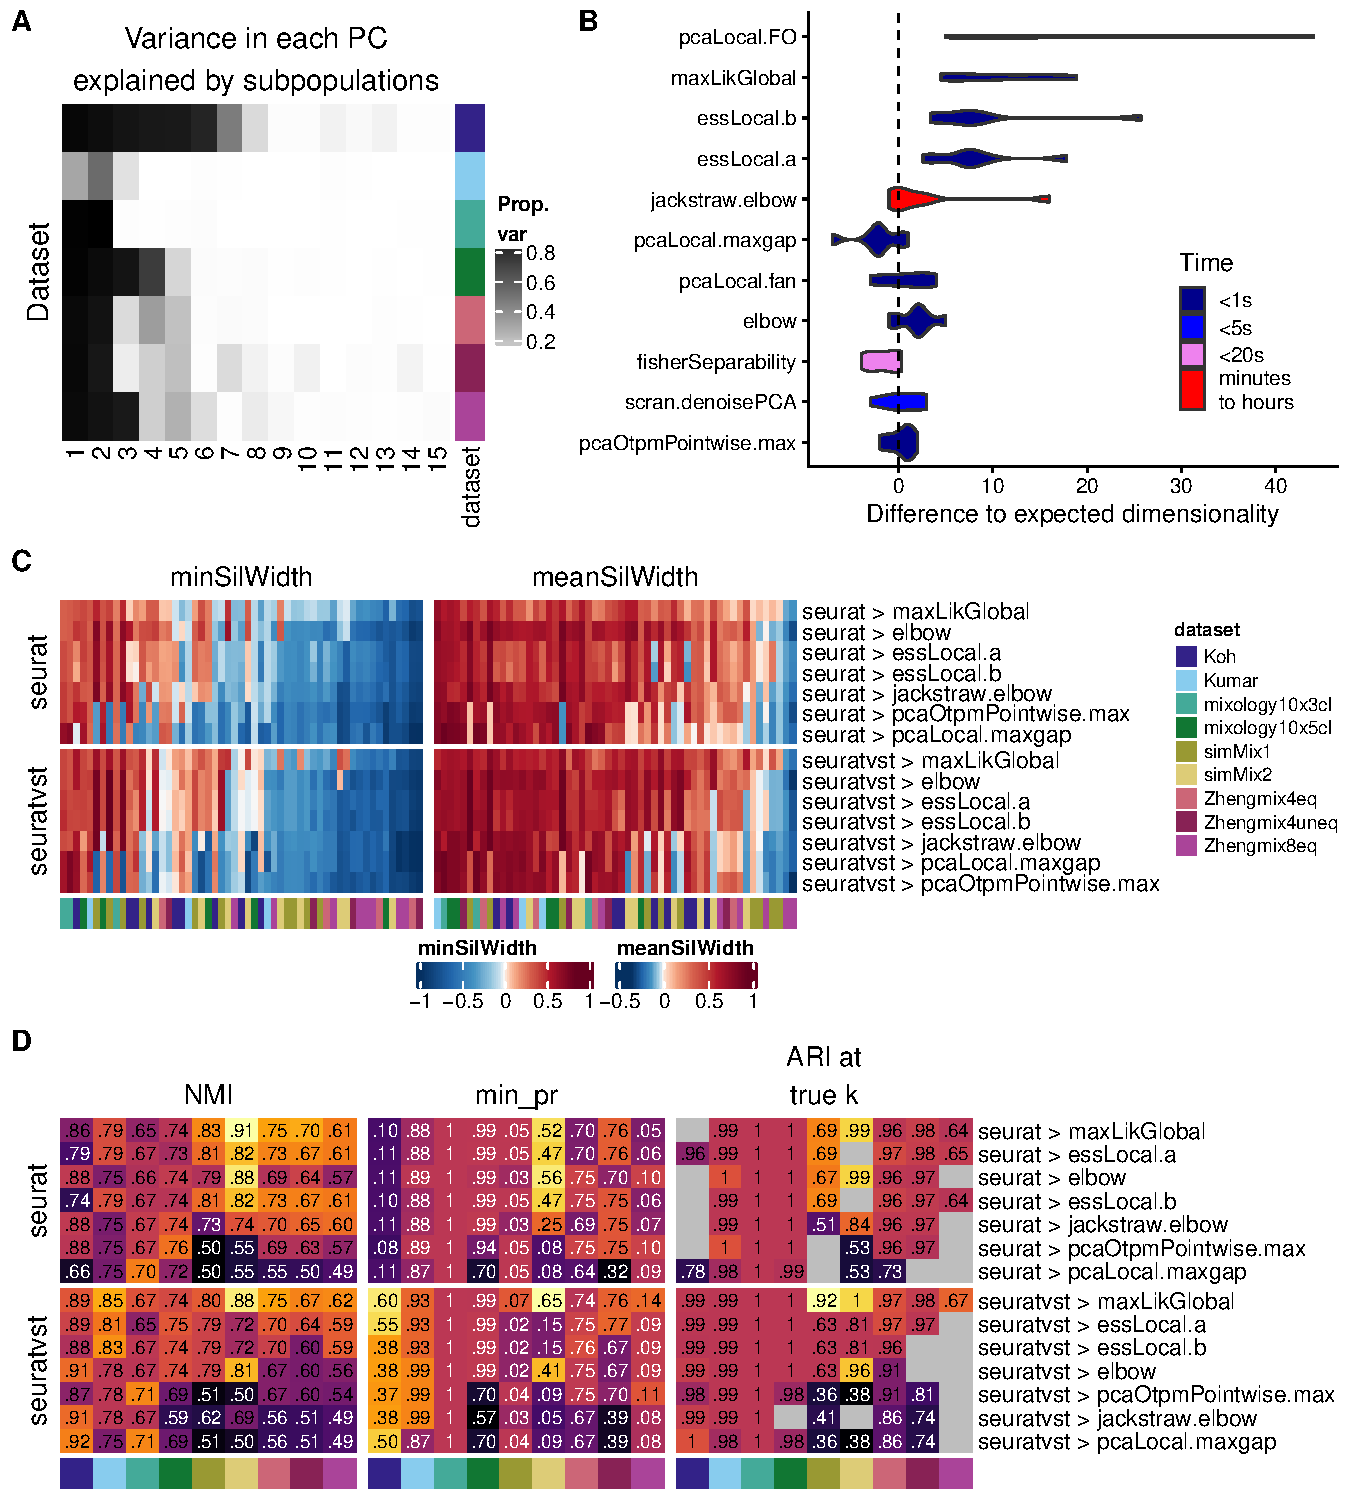
\includegraphics[scale=0.6, keepaspectratio]{{main_figures/dimensionality.pdf}}
    \caption{\textbf{Estimating dimensionality. A:} Estimated dimensionality using the proportion of variance in each component explained by the true subpopulations. \textbf{B:} Difference between `real' dimensionality (from \textbf{A}) and dimensionality estimation methods, along with computing time. \textbf{C:} Average silhouette width per subpopulation across a selection of methods, combined with \textit{sctransform} or standard \textit{Seurat} normalization. \textbf{D:} Clustering accuracy across the normalization/dimensionality estimation methods.}
    \label{fig:figure8}
\end{figure}



\begin{figure}
    \centering
    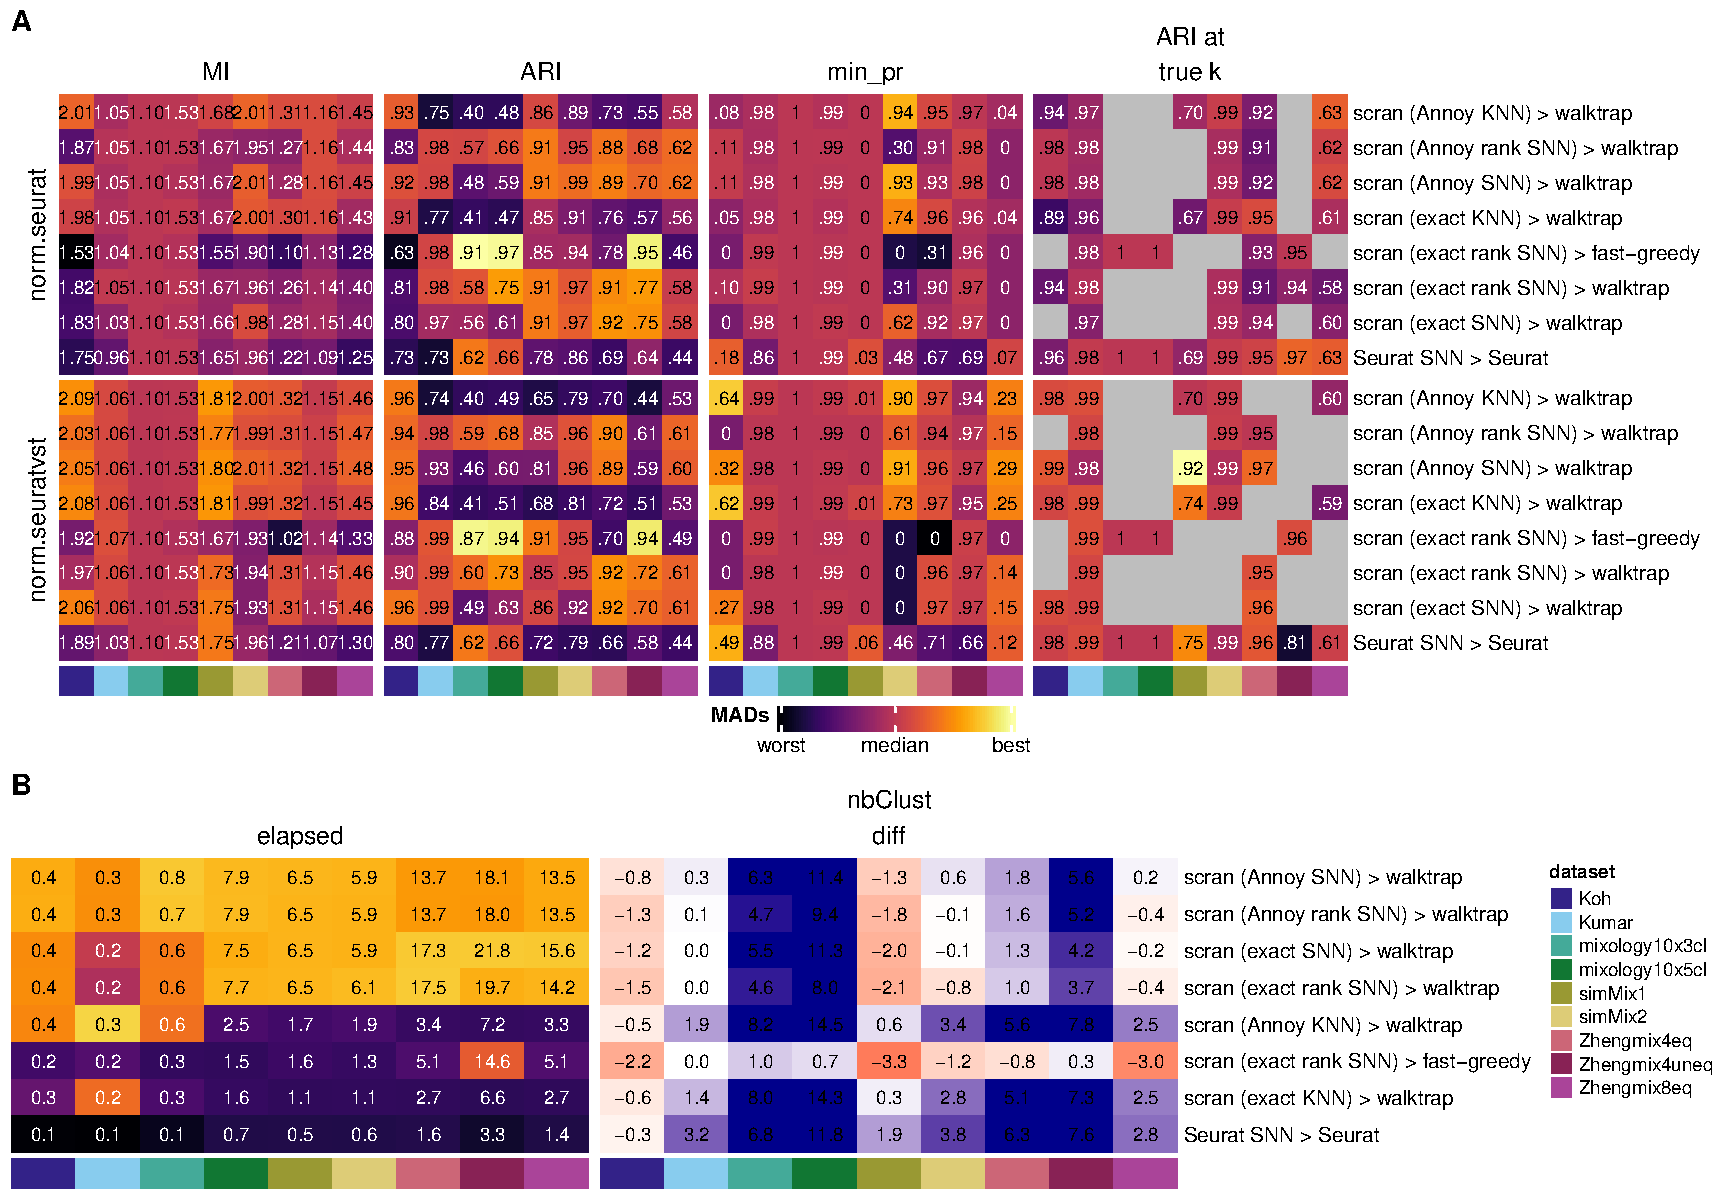
\includegraphics[scale=0.47, keepaspectratio]{{main_figures/clustering.pdf}}
    \caption{\textbf{Evaluation of clustering methods.} Clustering accuracy (\textbf{A}) and run time (\textbf{B}) of \textit{scran}- and \textit{Seurat}-based clustering tools in combination with \textit{sctransform} and standard \textit{Seurat}'s normalization.}
    \label{fig:figure9}
\end{figure}


\begin{figure}
    \centering
    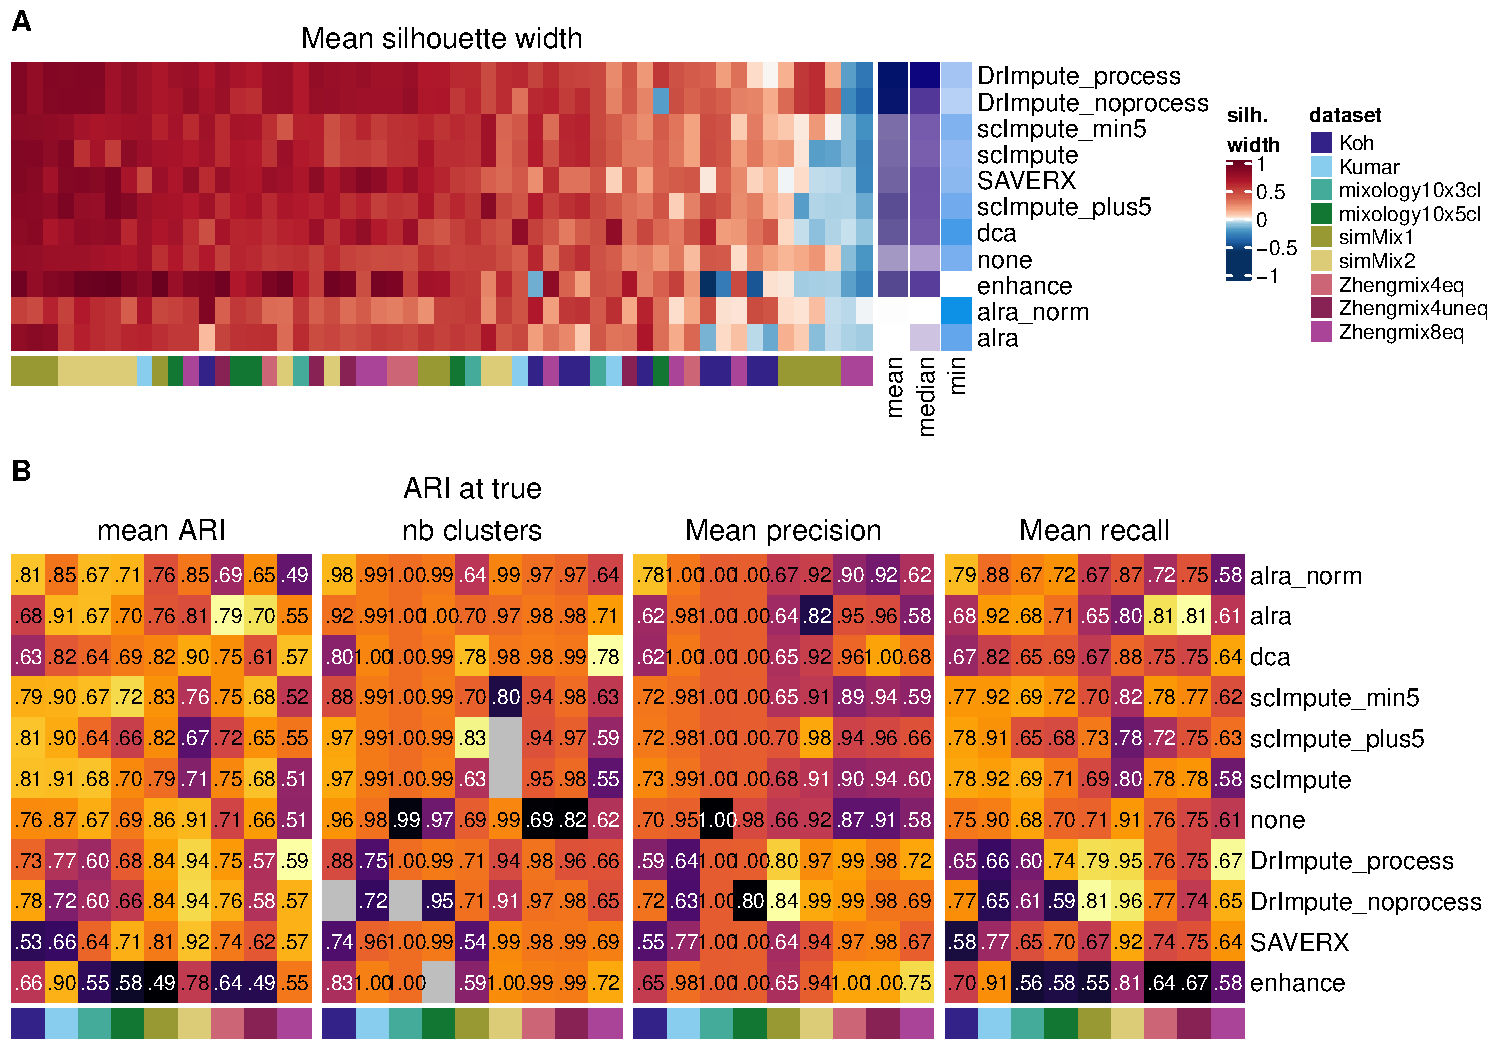
\includegraphics[scale=0.55, keepaspectratio]{{main_figures/imputation.pdf}}
     \caption{\textbf{Evaluation of imputation/denoising methods} Average silhouette width per subpopulation (\textbf{A}) and clustering accuracy (\textbf{B}) with or without (indicated as \textit{none}) application of a denoising/imputation method.}
    \label{fig:figure10}
\end{figure}


\begin{figure}[h]
    \centering
    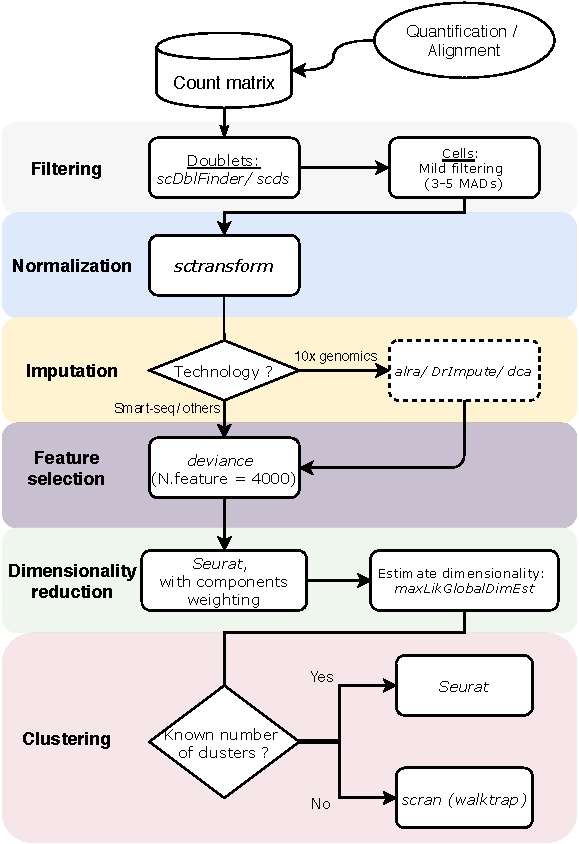
\includegraphics[scale=0.9,keepaspectratio]{main_figures/pipeComp_summary.pdf}
    \caption{\textbf{Recommendations of tools from filtering to clustering.}}
    \label{fig:figure11}
\end{figure}

\end{document}
